\documentclass{article}

\usepackage{graphicx}
\usepackage{rotating}
\usepackage{amsmath}
\usepackage{fancyhdr}
\usepackage{listings}
\usepackage{xcolor}
\usepackage{color}
\usepackage{textcomp}
\usepackage{float}
\usepackage{titlesec}
\usepackage[sorting=none]{biblatex}
\usepackage[margin=1in]{geometry}
\usepackage[font={small,it}]{caption}
\usepackage{placeins}
\usepackage{xepersian}

%\DeclareMathOperator*{\btie}{\bowtie}
\addbibresource{bibliography.bib}
\settextfont[Scale=1.2]{B-NAZANIN.TTF}
\setlatintextfont[Scale=1]{Times New Roman}
\renewcommand{\baselinestretch}{1.5}
\pagestyle{fancy}
\fancyhf{}
\rhead{پروژه‌ی سوم درس شبکه‌های کامپیوتری 2}
\lhead{\thepage}
\rfoot{علیرضا ابره فروش}
\lfoot{9816603}
\renewcommand{\headrulewidth}{1pt}
\renewcommand{\footrulewidth}{1pt}
%%%%%%%%%%
\lstset
{
    language=[latex]tex,
    basicstyle=\ttfamily,
    commentstyle=\color{black},
    columns=fullflexible,
    keepspaces=true,
    upquote=true,
    showstringspaces=false,
    morestring=[s]\\\%,
    stringstyle=\color{black},
}
%%%%%%%%%%
%beginMatlab
\definecolor{mygreen}{RGB}{28,172,0} % color values Red, Green, Blue
\definecolor{mylilas}{RGB}{170,55,241}
%endMatlab
\begin{document}
%beginMatlab
\lstset{language=Matlab,%
    %basicstyle=\color{red},
    breaklines=true,%
    morekeywords={matlab2tikz},
    keywordstyle=\color{blue},%
    morekeywords=[2]{1}, keywordstyle=[2]{\color{black}},
    identifierstyle=\color{black},%
    stringstyle=\color{mylilas},
    commentstyle=\color{mygreen},%
    showstringspaces=false,%without this there will be a symbol in the places where there is a space
    numbers=left,%
    numberstyle={\tiny \color{black}},% size of the numbers
    numbersep=9pt, % this defines how far the numbers are from the text
    emph=[1]{for,end,break},emphstyle=[1]\color{red}, %some words to emphasise
    %emph=[2]{word1,word2}, emphstyle=[2]{style},    
}
%endMatlab
\begin{titlepage}
\begin{center}

\includegraphics[width=0.4\textwidth]{figures/IUT Logo.png}\\
        
\LARGE
\textbf{دانشگاه صنعتی اصفهان}\\
\textbf{دانشکده مهندسی برق و کامپیوتر}\\
        
\vfill
        
\huge
\textbf{عنوان: تکلیف چهارم درس ریزپردازنده}\\
        
\vfill
        
\LARGE
\textbf{نام و نام خانوادگی: علیرضا ابره فروش}\\
\textbf{شماره دانشجویی: 9816603}\\
\textbf{نیم\,سال تحصیلی: پاییز 1400}\\
\textbf{مدرّس: دکتر عارف کریمی افشار}\\
\end{center}
\end{titlepage}


%\tableofcontents
\newpage


\section{}
\begin{figure}[H]
    \centering
    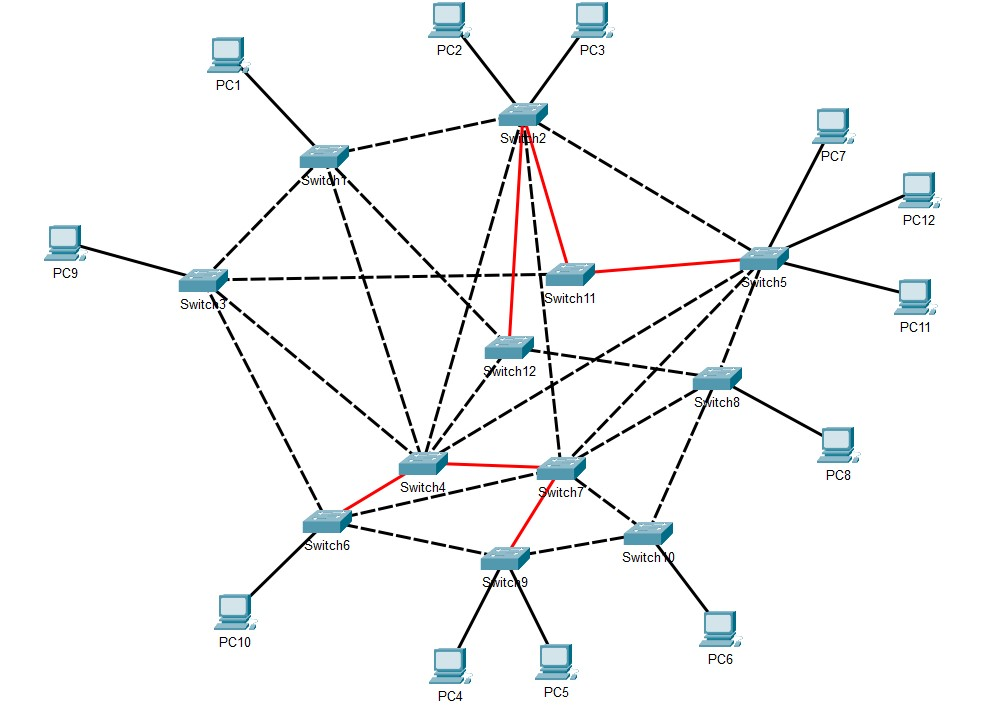
\includegraphics[width=1.0\textwidth]{figures/1.jpg}
    \caption
	{
سناریوی شامل 12 \lr{host} و 12 \lr{switch}
	}
    \label{fig:fig1}
\end{figure}

\section{}
\begin{figure}[H]
    \centering
    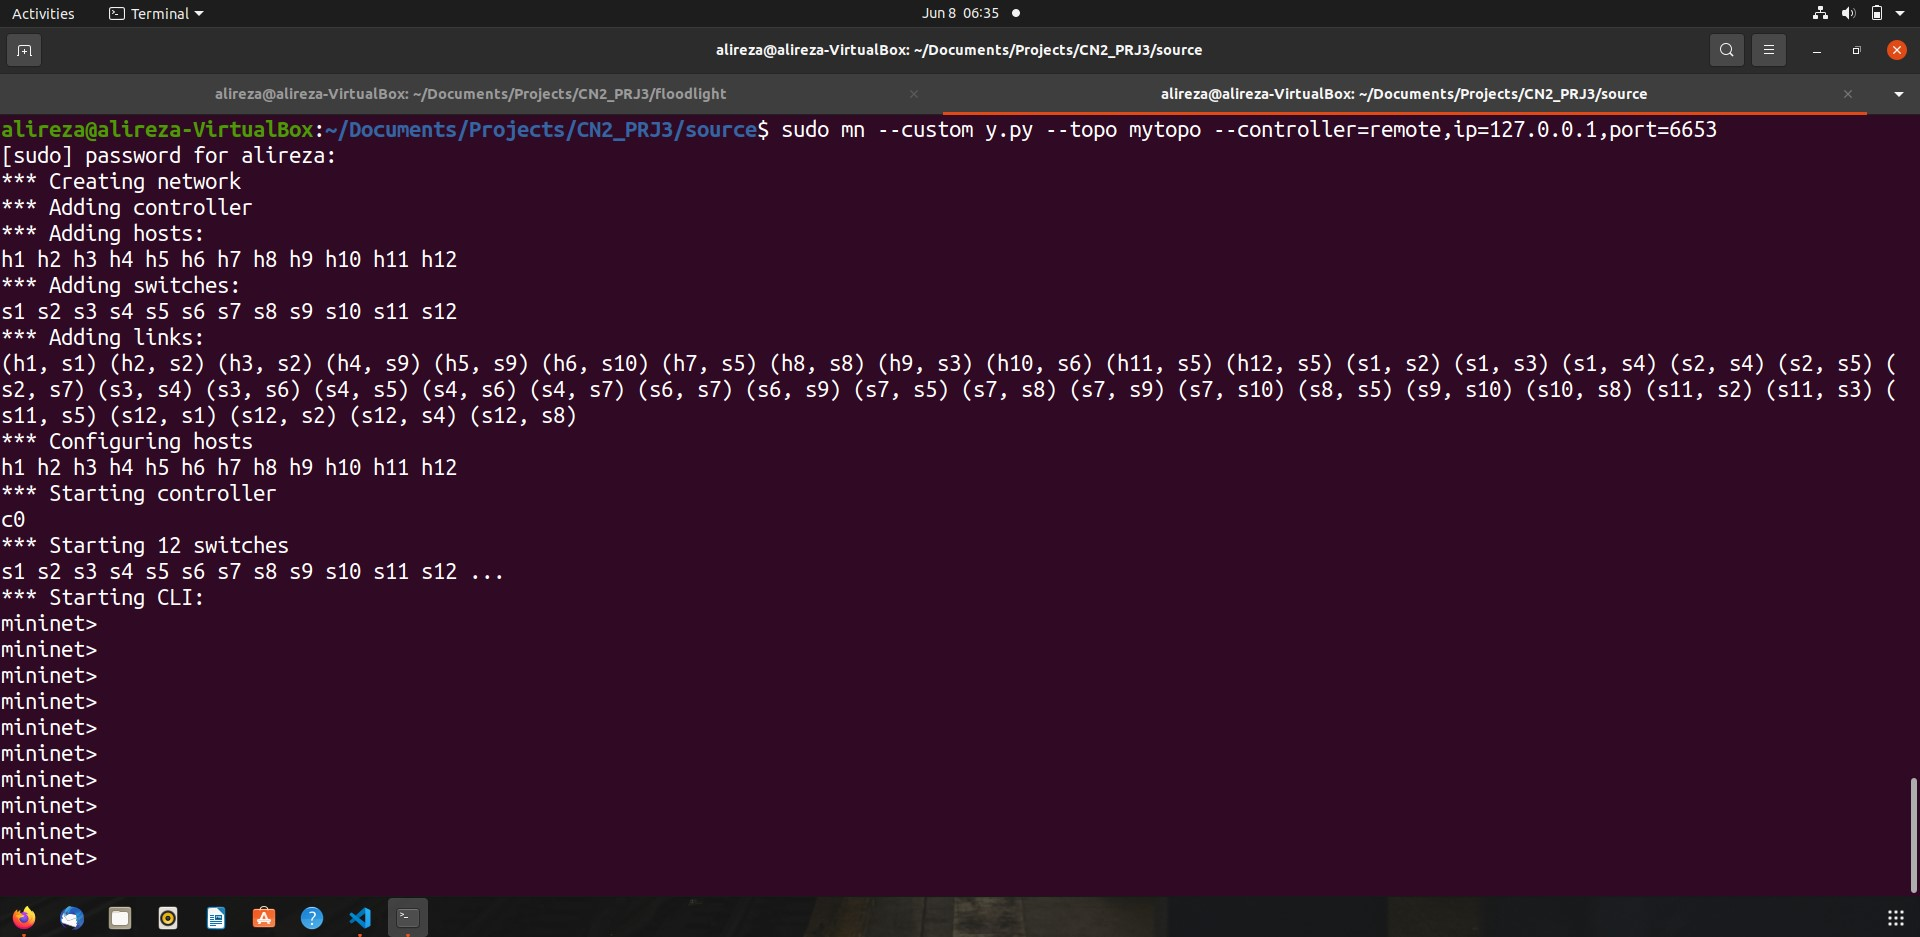
\includegraphics[width=1.0\textwidth]{figures/2b.jpg}
    \caption
	{
دستور اجرای توپولوژی دستی
	}
    \label{fig:fig1}
\end{figure}
\begin{figure}[H]
    \centering
    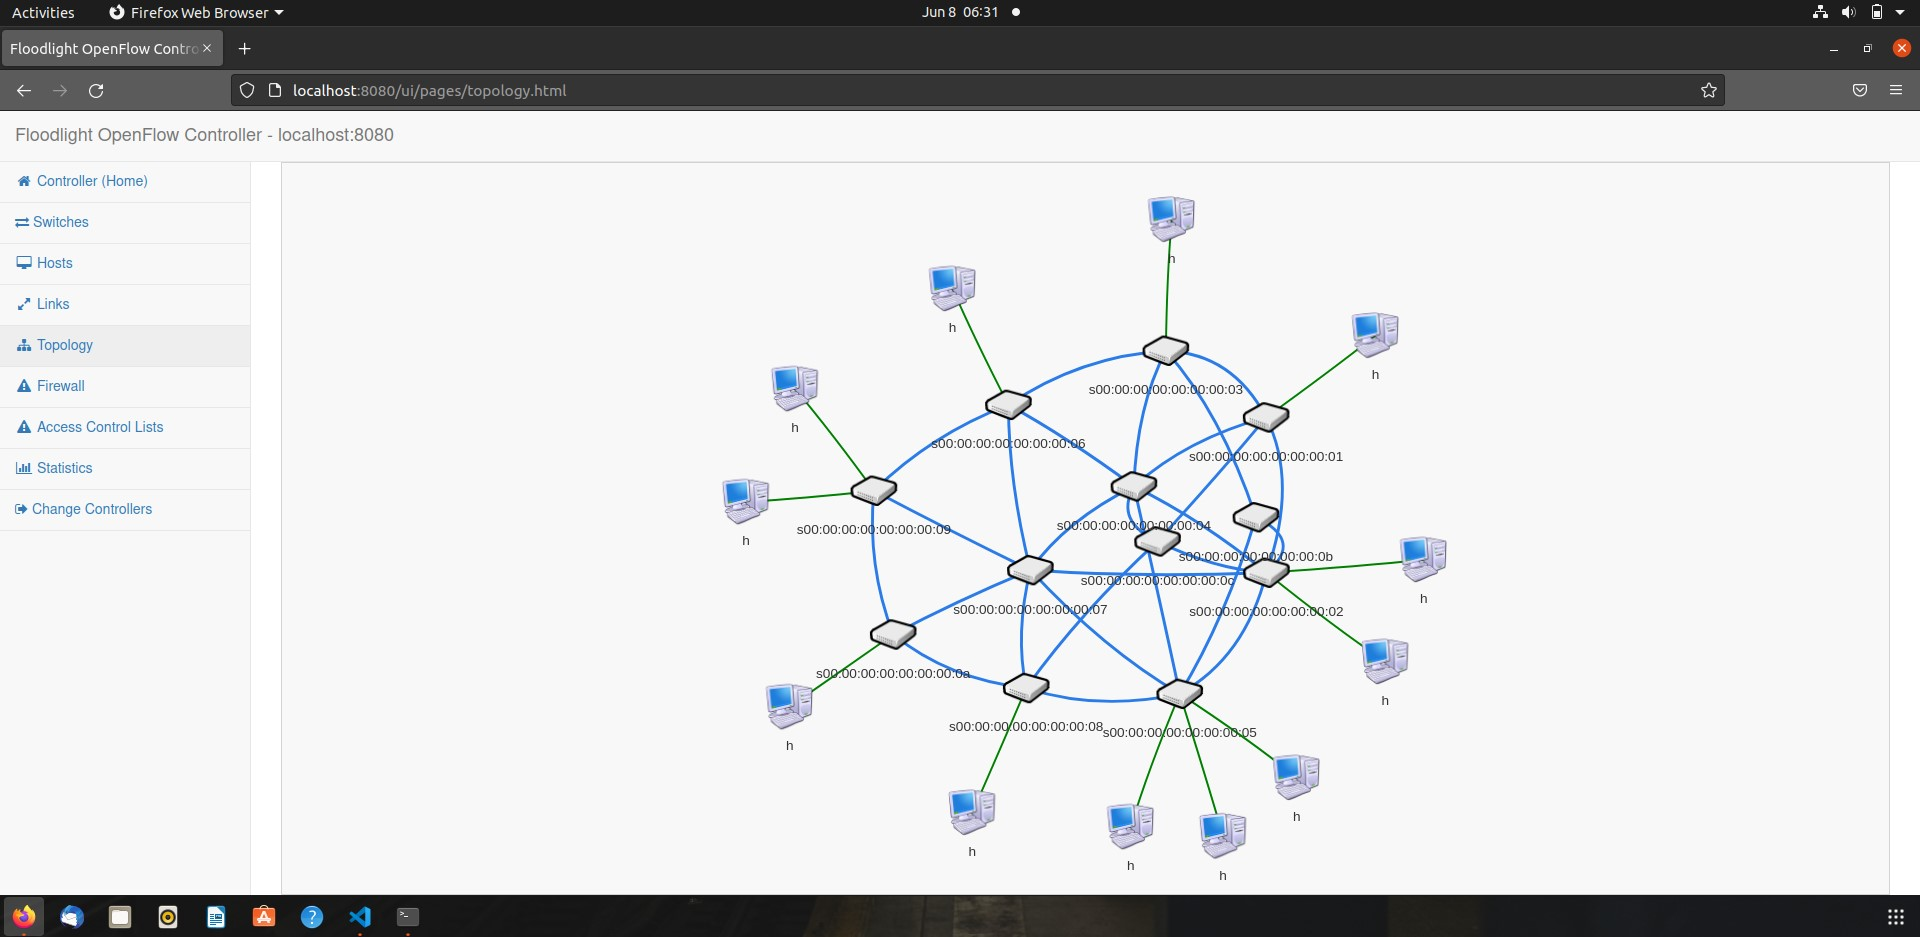
\includegraphics[width=1.0\textwidth]{figures/2a.jpg}
    \caption
	{
توپولوژی شبکه‌ی دستی ایجاد شده در \lr{mininet}
	}
    \label{fig:fig1}
\end{figure}

\section{}
همانطور که در خروجی دستورات \lr{ping} می‌بینیم، اتصال بین همه‌ی \lr{host}‌ها برقرار است.
\begin{figure}[H]
    \centering
    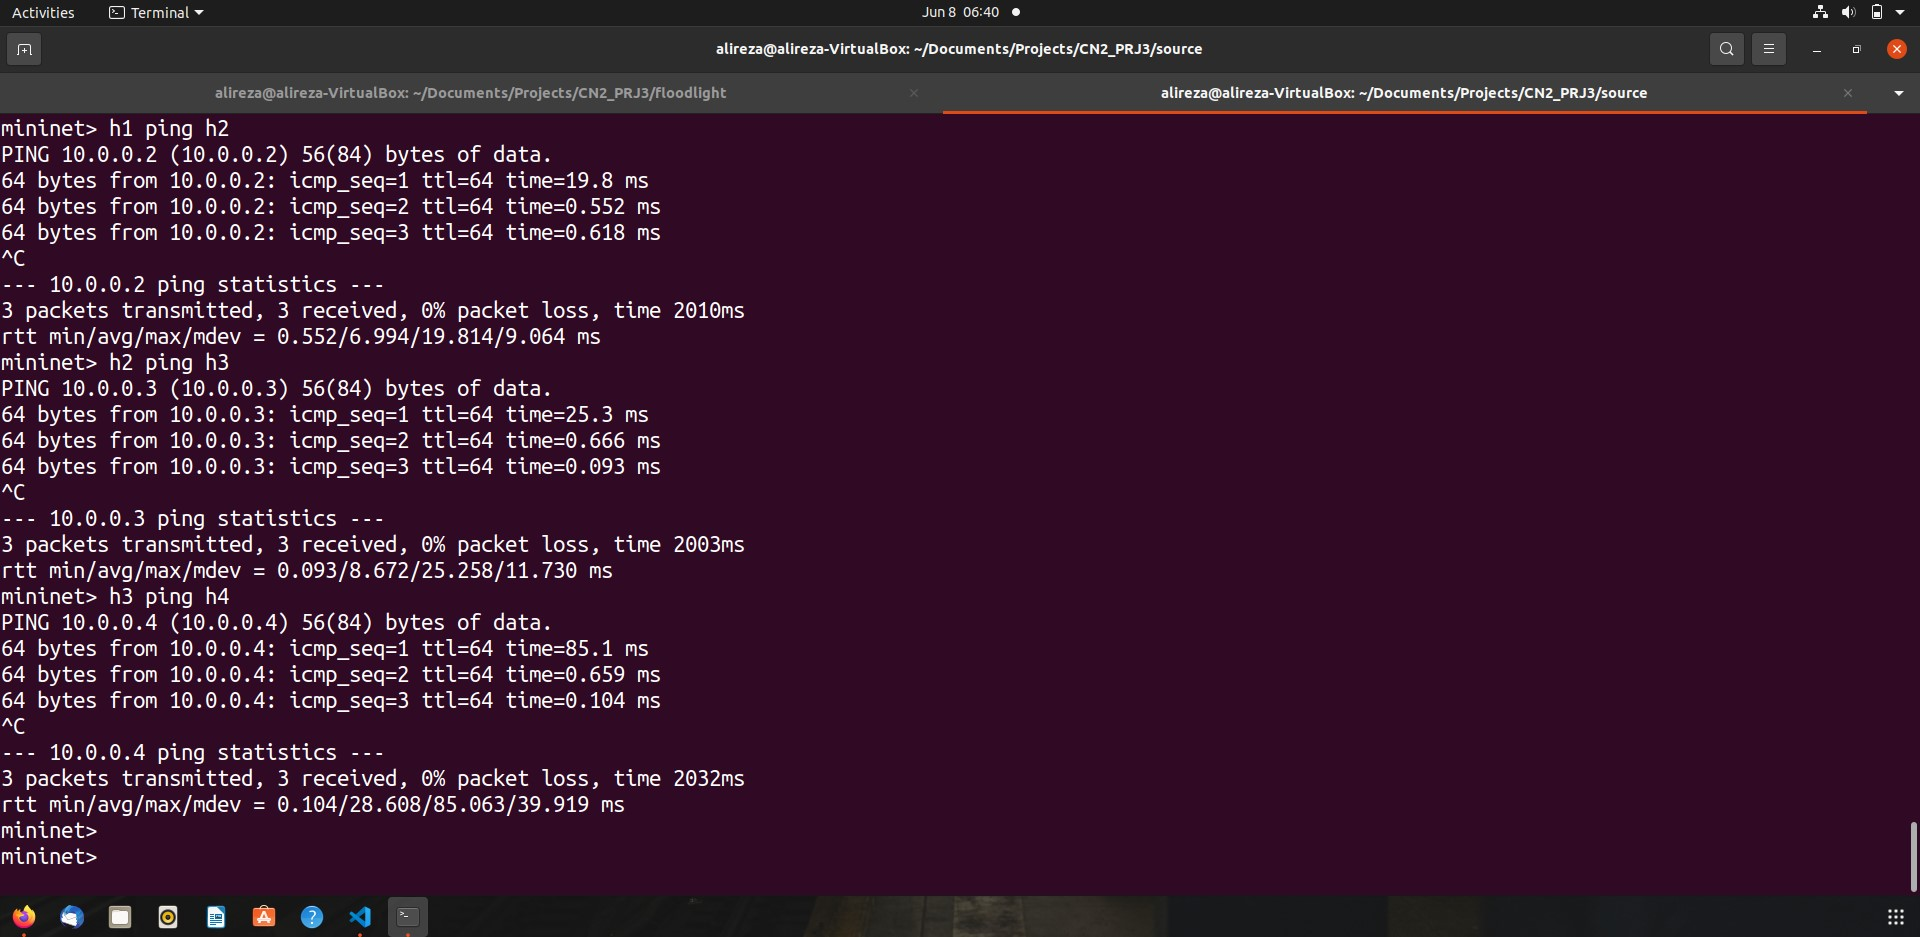
\includegraphics[width=1.0\textwidth]{figures/3.jpg}
    \caption
	{
خروجی دستور \lr{ping} برای چند تا از \lr{host}‌ها
	}
    \label{fig:fig1}
\end{figure}


\section{}
\begin{figure}[H]
    \centering
    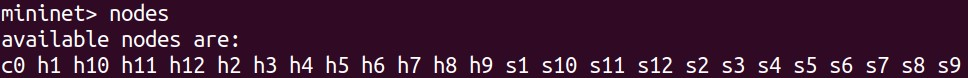
\includegraphics[width=1.0\textwidth]{figures/4a.jpg}
    \caption
	{
خروجی دستور \lr{nodes}
	}
    \label{fig:fig1}
\end{figure}
\begin{figure}[H]
    \centering
    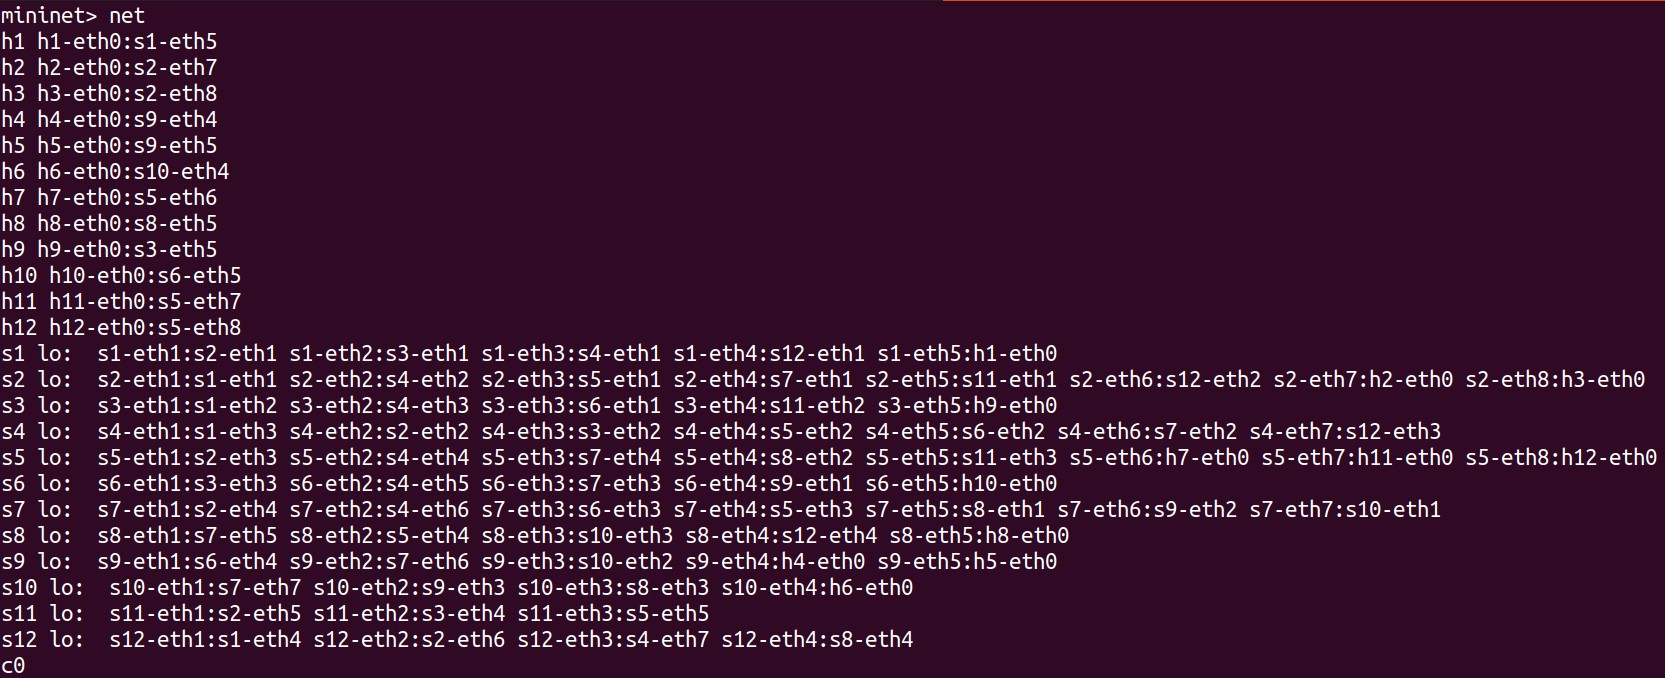
\includegraphics[width=1.0\textwidth]{figures/4b.jpg}
    \caption
	{
خروجی دستور \lr{net}
	}
    \label{fig:fig1}
\end{figure}
\begin{figure}[H]
    \centering
    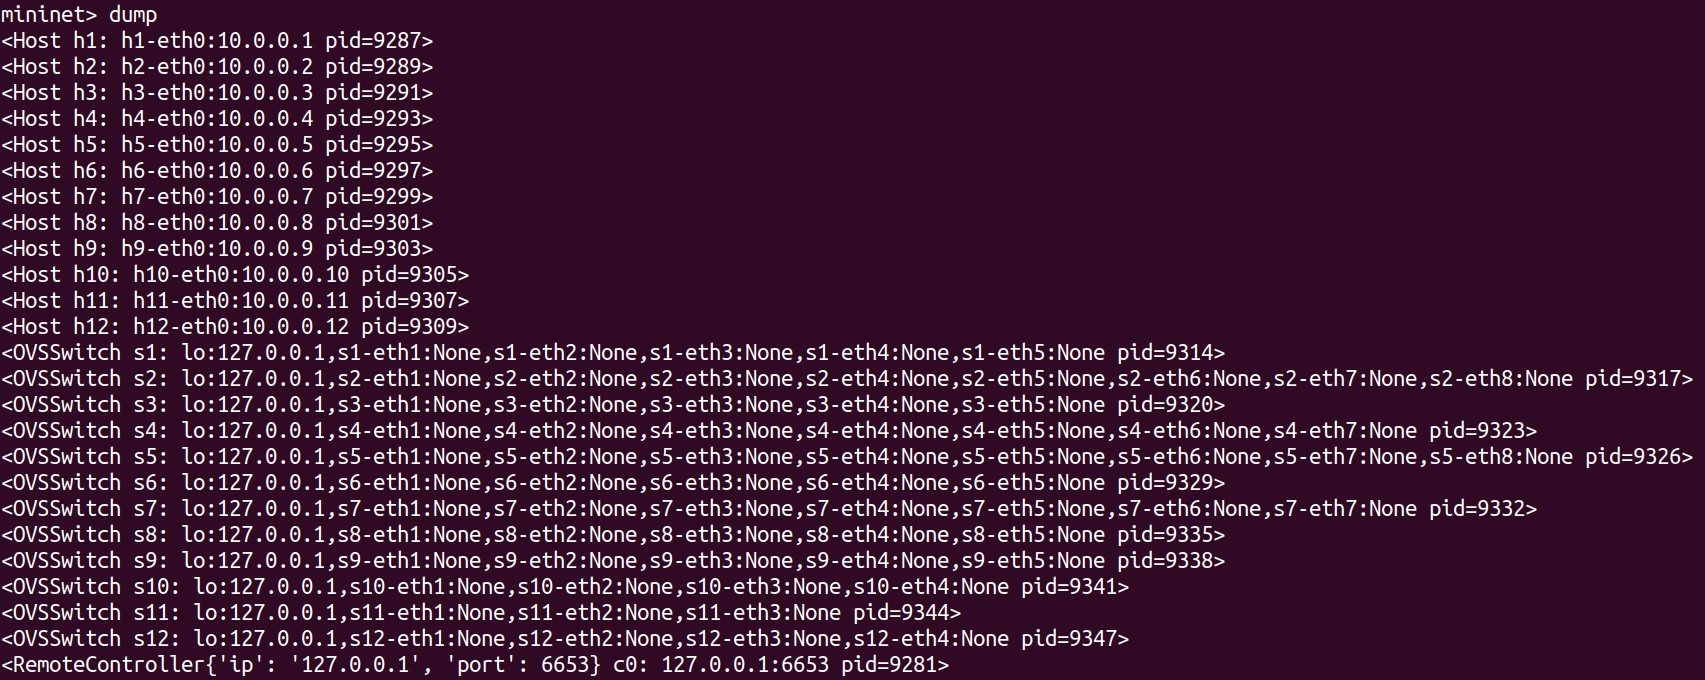
\includegraphics[width=1.0\textwidth]{figures/4c.jpg}
    \caption
	{
خروجی دستور \lr{dump}
	}
    \label{fig:fig1}
\end{figure}


\section{}
پهنای باند مسیرهای بین \lr{host}های 1 و 2، 2 و 3، 3 و 4، 8 و 9 به ترتیب برابر با
$11.4 Gbits/sec, 11.4 Gbits/sec$،
$13.9 Gbits/sec, 13.9 Gbits/sec$،
$11.2 Gbits/sec, 11.3 Gbits/sec$ و
$12.2 Gbits/sec, 12.2 Gbits/sec$ 
هستند.

\begin{figure}[H]
    \centering
    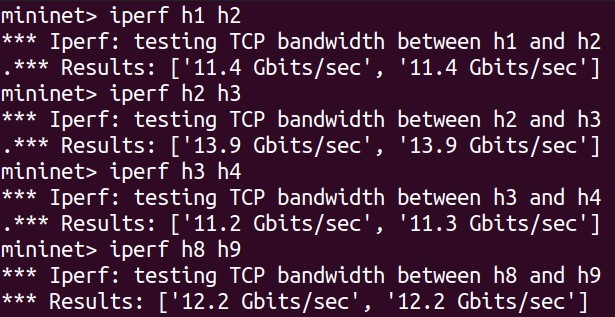
\includegraphics[width=1.0\textwidth]{figures/5.jpg}
    \caption
	{
خروجی دستور \lr{iperf} به ازای تعدادی از \lr{host}ها
	}
    \label{fig:fig1}
\end{figure}


\section{}
\begin{figure}[H]
    \centering
    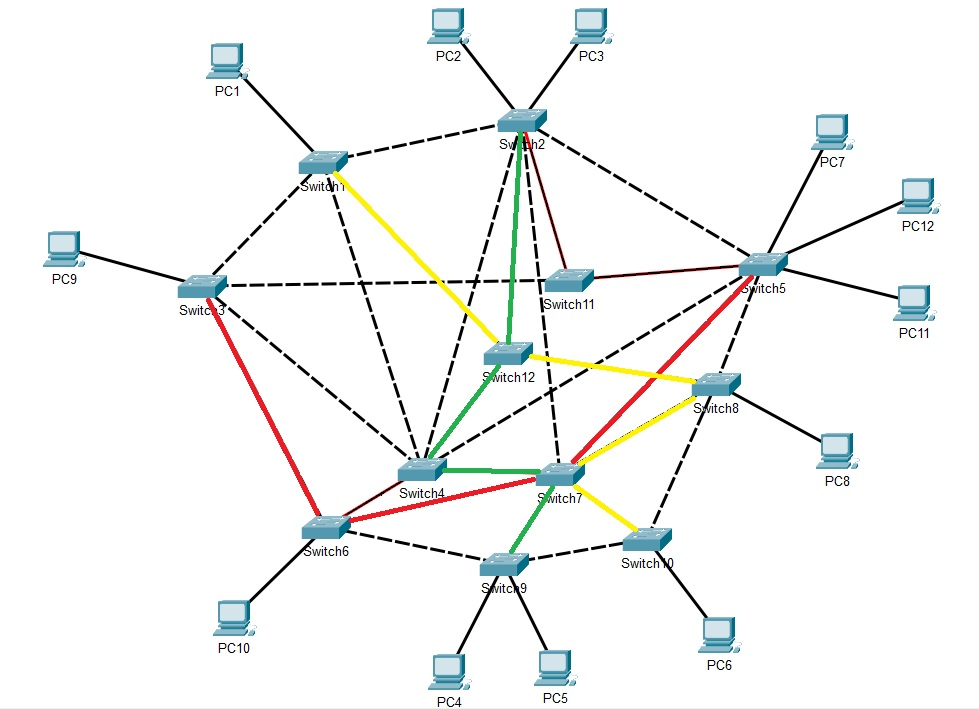
\includegraphics[width=1.0\textwidth]{figures/6.jpg}
    \caption
	{
مسیرهای سبز، قرمز و زرد
	}
    \label{fig:fig1}
\end{figure}

\section{}
\begin{figure}[H]
    \centering
    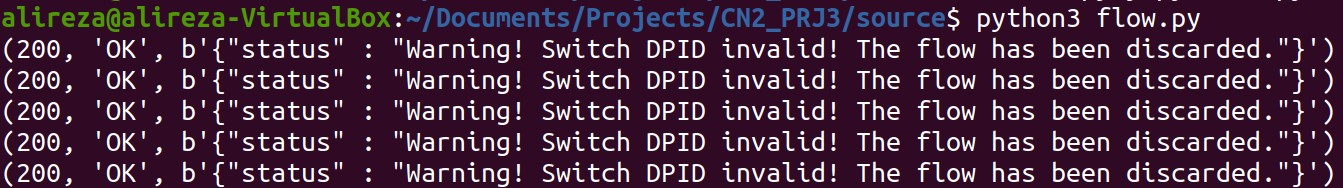
\includegraphics[width=1.0\textwidth]{figures/7.jpg}
    \caption
	{
خروجی پس از اجرای \lr{flow.py}
	}
    \label{fig:fig1}
\end{figure}
%%%%%%%%%%%%%%%%%%%%%%%%%%%%%%%%%%%





%%%%%%%%%%%

%\begin{figure}[H]
%    \centering
%    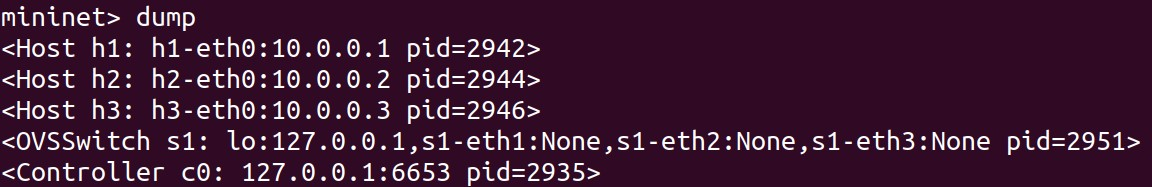
\includegraphics[width=1.0\textwidth]{figures/3f3.jpg}
%    \caption
%	{
%\lr{dump}
%	}
%    \label{fig:fig1}
%\end{figure}
%%%%%%%%%%%%%%%%%%%%%%%%%%%%%%%%%%%
%%%%%%%%%%%%%%%%%%%%%%%%%%%%%%%%%%%
%%%%%%%%%%%%%%%%%%%%%%%%%%%%%%%%%%%

\section*{منابع}
\renewcommand{\section}[2]{}%
\begin{thebibliography}{99} % assumes less than 100 references
%چنانچه مرجع فارسی نیز داشته باشید باید دستور فوق را فعال کنید و مراجع فارسی خود را بعد از این دستور وارد کنید


\begin{LTRitems}

\resetlatinfont

\bibitem{b1} http://mininet.org/overview/
\end{LTRitems}

\end{thebibliography}


\end{document}
